\documentclass[12pt,a4paper]{article}

% Packages
\usepackage{amsmath}
\usepackage{amssymb}
\usepackage{amsthm}
\usepackage[margin=1in]{geometry}
\usepackage{enumitem}
\usepackage{xcolor}
\usepackage{tikz}
\usetikzlibrary{arrows.meta}

% Custom environments
\newtheorem{explanation}{Explanation}
\theoremstyle{definition}
\newtheorem{solution}{Solution}

% Custom commands
\newcommand{\stage}[1]{\textbf{\textcolor{blue}{#1}}}
\newcommand{\critical}[1]{\textbf{\textcolor{red}{#1}}}

% Title information
\title{Exercise Sheet 1, Question 6: Existence and Uniqueness\\
Methods of Applied Mathematics [SEMT30006]}
\author{}
\date{}

\begin{document}

\maketitle

\section*{Problem Statement}

Solve the following initial value problems to find a solution $x(t)$ in terms of $x_0$:

\begin{enumerate}[label=(\alph*)]
    \item $\dot{x} = x^2$ with $x(0) = x_0$
    \item $\dot{x} = |x|$ with $x(0) = x_0$
    \item $\dot{x} = |x|^{1/2}$ with $x(0) = x_0$
\end{enumerate}

Then answer the following questions for each system:

\begin{enumerate}[label=(\roman*)]
    \item Consider three initial conditions $x_0 = 0$, $x_0 = -1$ and $x_0 = +1$. From each, where does the solution go and how long does it take?
    \item Identify the different orbits of each system.
    \item Are the orbits uniquely determined by the ODE (for a given $x_0$ is there only one unique solution)?
    \item Show that each system is/isn't Lipschitz continuous, and say how this agrees with your answer to (iii).
\end{enumerate}

\section*{Theoretical Framework: Existence and Uniqueness}

\begin{explanation}[Picard-Lindelöf Theorem]
For the initial value problem $\dot{x} = f(x, t)$ with $x(t_0) = x_0$:

\textbf{Existence:} If $f$ is continuous, then a solution exists locally.

\textbf{Uniqueness:} If $f$ is Lipschitz continuous in $x$, then the solution is unique.

\textbf{Lipschitz Condition:} A function $f(x)$ is Lipschitz continuous if there exists a constant $L > 0$ such that:
$$|f(x_1) - f(x_2)| \leq L|x_1 - x_2| \quad \text{for all } x_1, x_2$$

Equivalently, if $f$ is differentiable and $|f'(x)|$ is bounded, then $f$ is Lipschitz.
\end{explanation}

\critical{KEY INSIGHT:} When Lipschitz condition fails (e.g., $f'(x)$ unbounded), uniqueness can fail. We may have multiple solutions from the same initial condition!

\newpage

\section{Part (a): $\dot{x} = x^2$ with $x(0) = x_0$}

\subsection*{Solving the ODE}

\begin{solution}

\textbf{Step 1: Separate Variables}

The equation $\dot{x} = x^2$ is separable. For $x \neq 0$:
$$\frac{dx}{dt} = x^2 \quad \Rightarrow \quad \frac{dx}{x^2} = dt$$

\textbf{Step 2: Integrate Both Sides}

$$\int \frac{dx}{x^2} = \int dt$$

$$-\frac{1}{x} = t + C$$

\textbf{Step 3: Apply Initial Condition}

At $t = 0$: $x(0) = x_0$

$$-\frac{1}{x_0} = 0 + C \quad \Rightarrow \quad C = -\frac{1}{x_0}$$

Therefore:
$$-\frac{1}{x} = t - \frac{1}{x_0}$$

\textbf{Step 4: Solve for $x(t)$}

$$\frac{1}{x} = \frac{1}{x_0} - t = \frac{1 - x_0 t}{x_0}$$

$$\boxed{x(t) = \frac{x_0}{1 - x_0 t}}$$

\begin{explanation}[Special Case: $x_0 = 0$]
If $x_0 = 0$, then $\dot{x} = 0^2 = 0$, so:
$$\boxed{x(t) = 0 \quad \text{for all } t}$$

This is the trivial solution (constant at origin).
\end{explanation}

\end{solution}

\vspace{10pt}
\hrule
\vspace{10pt}

\subsection*{(i) Behavior for Three Initial Conditions}

\begin{solution}

\textbf{Case 1: $x_0 = 0$}

$$x(t) = 0 \quad \text{for all } t$$

\begin{itemize}
    \item \textbf{Where does it go?} Stays at $x = 0$ forever
    \item \textbf{How long?} Remains there for all time $t \in (-\infty, \infty)$
    \item \textbf{Nature:} Equilibrium solution
\end{itemize}

\textbf{Case 2: $x_0 = -1$}

$$x(t) = \frac{-1}{1 - (-1)t} = \frac{-1}{1 + t}$$

\begin{itemize}
    \item At $t = 0$: $x = -1$
    \item As $t \to \infty$: $x(t) \to 0^-$ (approaches zero from below)
    \item As $t \to -1^+$: $x(t) \to -\infty$ (blows up to $-\infty$ as $t$ approaches $-1$ from right)
    \item \textbf{Where does it go?} Approaches $x = 0$ as $t \to +\infty$
    \item \textbf{How long?} Takes infinite time to reach $x = 0$
\end{itemize}

\begin{explanation}[Why Approaches Zero]
For $x_0 < 0$, we have $x(t) = \frac{x_0}{1 - x_0 t}$ where $1 - x_0 t > 1$ for $t > 0$.

Since $|x_0| < 1 - x_0 t$ for positive $t$:
$$|x(t)| = \frac{|x_0|}{1 - x_0 t} < |x_0| \quad \text{and decreases as } t \to \infty$$
\end{explanation}

\textbf{Case 3: $x_0 = +1$}

$$x(t) = \frac{1}{1 - t}$$

\begin{itemize}
    \item At $t = 0$: $x = 1$
    \item As $t \to 1^-$: $x(t) \to +\infty$ (blows up to $+\infty$)
    \item \textbf{Where does it go?} Diverges to $+\infty$
    \item \textbf{How long?} Reaches $+\infty$ at time $t = 1$ (finite-time blow-up!)
    \item Solution only exists on $t \in (-\infty, 1)$
\end{itemize}

\begin{explanation}[Finite-Time Blow-Up]
The solution becomes singular at $t = t^* = \frac{1}{x_0}$ when $x_0 > 0$:
$$x(t) = \frac{x_0}{1 - x_0 t} \to \infty \quad \text{as } t \to \frac{1}{x_0}$$

For $x_0 = 1$: blow-up time is $t^* = 1$

This is characteristic of super-linear growth ($\dot{x} = x^2$).
\end{explanation}

\textbf{Summary:}

\begin{center}
\begin{tabular}{|c|c|c|}
\hline
$x_0$ & Long-time behavior & Time to destination \\
\hline
$0$ & Stays at $x = 0$ & All time \\
\hline
$-1$ & $x(t) \to 0$ as $t \to \infty$ & Infinite time \\
\hline
$+1$ & $x(t) \to +\infty$ as $t \to 1$ & Finite time ($t^* = 1$) \\
\hline
\end{tabular}
\end{center}

\end{solution}

\vspace{10pt}
\hrule
\vspace{10pt}

\subsection*{(ii) Different Orbits}

\begin{solution}

An \textbf{orbit} is the trajectory $x(t)$ in phase space (here, the $x$-axis).

\textbf{Classification of Orbits:}

\textbf{Type 1: Equilibrium Orbit}
$$x(t) = 0 \quad \text{for all } t$$
Starting point: $x_0 = 0$

\textbf{Type 2: Monotonic Decay to Zero ($x_0 < 0$)}
$$x(t) = \frac{x_0}{1 - x_0 t} \quad \text{with } x_0 < 0$$
\begin{itemize}
    \item Solution exists for all $t > 0$
    \item $x(t)$ increases (becomes less negative) toward $0$
    \item $x(t) \to 0$ as $t \to \infty$
    \item Example: $x_0 = -1$ gives $x(t) = \frac{-1}{1+t}$
\end{itemize}

\textbf{Type 3: Finite-Time Blow-Up ($x_0 > 0$)}
$$x(t) = \frac{x_0}{1 - x_0 t} \quad \text{with } x_0 > 0$$
\begin{itemize}
    \item Solution exists only on $t \in (-\infty, 1/x_0)$
    \item $x(t)$ increases without bound
    \item $x(t) \to +\infty$ as $t \to (1/x_0)^-$
    \item Blow-up time: $t^* = \frac{1}{x_0}$
    \item Example: $x_0 = 1$ gives $x(t) = \frac{1}{1-t}$ with $t^* = 1$
\end{itemize}

\begin{explanation}[Phase Portrait]
On the phase line:
\begin{itemize}
    \item Equilibrium at $x = 0$ (semi-stable: attracts from left, repels to right)
    \item For $x < 0$: flow toward zero ($\dot{x} = x^2 > 0$ means increasing)
    \item For $x > 0$: flow away from zero ($\dot{x} = x^2 > 0$ means increasing)
\end{itemize}

\begin{center}
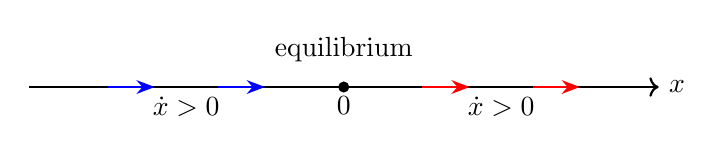
\begin{tikzpicture}[scale=2]
    \draw[->,thick] (-2,0) -- (2,0) node[right] {$x$};
    \fill[black] (0,0) circle (1pt) node[below] {$0$};
    \node[above] at (0,0.1) {equilibrium};

    % Flow arrows
    \draw[-{Stealth},thick,blue] (-1.5,0) -- (-1.2,0);
    \draw[-{Stealth},thick,blue] (-0.8,0) -- (-0.5,0);
    \node[below] at (-1,0) {$\dot{x} > 0$};

    \draw[-{Stealth},thick,red] (0.5,0) -- (0.8,0);
    \draw[-{Stealth},thick,red] (1.2,0) -- (1.5,0);
    \node[below] at (1,0) {$\dot{x} > 0$};
\end{tikzpicture}
\end{center}

Note: Both sides have $\dot{x} > 0$ because $x^2$ is always positive (except at $x=0$).
\end{explanation}

\textbf{Summary:} Three distinct types of orbits based on initial condition.

\end{solution}

\vspace{10pt}
\hrule
\vspace{10pt}

\subsection*{(iii) Uniqueness of Orbits}

\begin{solution}

\textbf{Question:} For a given $x_0$, is there only one solution?

\textbf{Answer:} \boxed{\text{YES - solutions are unique}}

\begin{explanation}[Why Uniqueness Holds]
From any initial condition $x_0$, there is exactly one solution:
\begin{itemize}
    \item If $x_0 = 0$: unique solution $x(t) = 0$
    \item If $x_0 \neq 0$: unique solution $x(t) = \frac{x_0}{1 - x_0 t}$
\end{itemize}

We derived these solutions using separation of variables, which gives a unique solution (up to the domain of existence).

The only subtlety is at $x_0 = 0$, where we cannot divide by $x^2$. But directly from the ODE: if $x(0) = 0$, then $\dot{x}(0) = 0^2 = 0$, so the solution must remain at $x = 0$.

\critical{NO NON-UNIQUENESS:} Unlike part (c), this system has unique solutions from every initial condition.
\end{explanation}

\end{solution}

\vspace{10pt}
\hrule
\vspace{10pt}

\subsection*{(iv) Lipschitz Continuity}

\begin{solution}

\textbf{Question:} Is $f(x) = x^2$ Lipschitz continuous?

\textbf{Step 1: Check Lipschitz Condition}

For $f(x) = x^2$, compute the derivative:
$$f'(x) = 2x$$

\textbf{Step 2: Is $|f'(x)|$ Bounded?}

$$|f'(x)| = |2x| = 2|x|$$

This is \textbf{NOT bounded} as $x \to \pm\infty$.

Therefore, $f(x) = x^2$ is \textbf{NOT globally Lipschitz continuous}.

\textbf{Step 3: Local Lipschitz Continuity}

However, on any bounded interval $|x| \leq M$:
$$|f'(x)| = 2|x| \leq 2M$$

So $f$ is Lipschitz continuous on any compact set with Lipschitz constant $L = 2M$.

\boxed{\text{Locally Lipschitz, but NOT globally Lipschitz}}

\begin{explanation}[Lipschitz vs. Uniqueness]
Despite $f(x) = x^2$ not being globally Lipschitz, we still have uniqueness!

Why? The Picard-Lindelöf theorem says:
\begin{itemize}
    \item Lipschitz $\Rightarrow$ Uniqueness (sufficient condition)
    \item But uniqueness can hold even without global Lipschitz (not necessary)
\end{itemize}

\textbf{Local Lipschitz is enough:} Since $f(x) = x^2$ is locally Lipschitz, and solutions remain in compact regions over finite time, uniqueness holds locally. As long as we haven't reached blow-up, uniqueness is guaranteed.

\textbf{What about blow-up?} The finite-time blow-up for $x_0 > 0$ doesn't violate uniqueness—the solution simply ceases to exist beyond $t^* = 1/x_0$. There's still only one solution on $[0, t^*)$.
\end{explanation}

\textbf{Agreement with (iii):}

\begin{itemize}
    \item Uniqueness holds $\checkmark$
    \item Local Lipschitz condition guarantees this $\checkmark$
    \item Lack of global Lipschitz doesn't prevent uniqueness $\checkmark$
    \item Finite-time blow-up is consistent with local uniqueness $\checkmark$
\end{itemize}

\end{solution}

\newpage

\section{Part (b): $\dot{x} = |x|$ with $x(0) = x_0$}

\subsection*{Solving the ODE}

\begin{solution}

\textbf{Step 1: Case Analysis}

Since $|x|$ has different forms depending on sign of $x$, we solve separately:

$$|x| = \begin{cases}
x & \text{if } x \geq 0 \\
-x & \text{if } x < 0
\end{cases}$$

\textbf{Case 1: $x > 0$}

$$\frac{dx}{dt} = x \quad \Rightarrow \quad \frac{dx}{x} = dt$$

Integrating:
$$\ln|x| = t + C \quad \Rightarrow \quad x = Ae^t$$

With $x(0) = x_0 > 0$: $A = x_0$

$$\boxed{x(t) = x_0 e^t \quad \text{for } x_0 > 0}$$

\textbf{Case 2: $x < 0$}

$$\frac{dx}{dt} = -x \quad \Rightarrow \quad \frac{dx}{x} = -dt$$

Integrating:
$$\ln|x| = -t + C \quad \Rightarrow \quad x = -Be^{-t}$$

With $x(0) = x_0 < 0$: $-B = x_0$, so $B = -x_0 > 0$

$$\boxed{x(t) = x_0 e^{-t} \quad \text{for } x_0 < 0}$$

\textbf{Case 3: $x = 0$}

If $x(0) = 0$, then $\dot{x} = |0| = 0$, so:
$$\boxed{x(t) = 0 \quad \text{for all } t}$$

\textbf{Complete Solution:}

$$\boxed{x(t) = \begin{cases}
x_0 e^t & \text{if } x_0 > 0 \\
0 & \text{if } x_0 = 0 \\
x_0 e^{-t} & \text{if } x_0 < 0
\end{cases}}$$

\begin{explanation}[Verification]
Check each case satisfies $\dot{x} = |x|$:
\begin{itemize}
    \item If $x_0 > 0$: $x = x_0 e^t > 0$, so $\dot{x} = x_0 e^t = x = |x|$ ✓
    \item If $x_0 = 0$: $x = 0$, so $\dot{x} = 0 = |0|$ ✓
    \item If $x_0 < 0$: $x = x_0 e^{-t} < 0$, so $\dot{x} = -x_0 e^{-t} = -x = |x|$ ✓
\end{itemize}
\end{explanation}

\end{solution}

\vspace{10pt}
\hrule
\vspace{10pt}

\subsection*{(i) Behavior for Three Initial Conditions}

\begin{solution}

\textbf{Case 1: $x_0 = 0$}

$$x(t) = 0 \quad \text{for all } t$$

\begin{itemize}
    \item \textbf{Where does it go?} Stays at $x = 0$ forever
    \item \textbf{How long?} Remains there for all time
    \item \textbf{Nature:} Equilibrium solution
\end{itemize}

\textbf{Case 2: $x_0 = -1$}

$$x(t) = -e^{-t}$$

\begin{itemize}
    \item At $t = 0$: $x = -1$
    \item As $t \to \infty$: $x(t) = -e^{-t} \to 0^-$ (approaches zero from below)
    \item Exponential decay toward zero
    \item \textbf{Where does it go?} Approaches $x = 0$
    \item \textbf{How long?} Infinite time (asymptotic approach)
\end{itemize}

\textbf{Case 3: $x_0 = +1$}

$$x(t) = e^t$$

\begin{itemize}
    \item At $t = 0$: $x = 1$
    \item As $t \to \infty$: $x(t) = e^t \to +\infty$
    \item Exponential growth
    \item \textbf{Where does it go?} Diverges to $+\infty$
    \item \textbf{How long?} Infinite time (but grows unboundedly)
    \item Solution exists for all $t \in (-\infty, \infty)$
\end{itemize}

\begin{explanation}[Comparison to Part (a)]
Unlike part (a):
\begin{itemize}
    \item NO finite-time blow-up (exponential growth is slower than $x^2$ growth)
    \item Solutions from $x_0 < 0$ decay exponentially (not algebraically)
    \item Solutions from $x_0 > 0$ grow exponentially (no singularity)
\end{itemize}
\end{explanation}

\textbf{Summary:}

\begin{center}
\begin{tabular}{|c|c|c|}
\hline
$x_0$ & Long-time behavior & Time to destination \\
\hline
$0$ & Stays at $x = 0$ & All time \\
\hline
$-1$ & $x(t) \to 0$ as $t \to \infty$ & Infinite time \\
\hline
$+1$ & $x(t) \to +\infty$ as $t \to \infty$ & Infinite time \\
\hline
\end{tabular}
\end{center}

\end{solution}

\vspace{10pt}
\hrule
\vspace{10pt}

\subsection*{(ii) Different Orbits}

\begin{solution}

\textbf{Classification of Orbits:}

\textbf{Type 1: Equilibrium Orbit}
$$x(t) = 0 \quad \text{for all } t$$
Starting point: $x_0 = 0$

\textbf{Type 2: Exponential Decay to Zero ($x_0 < 0$)}
$$x(t) = x_0 e^{-t} \quad \text{with } x_0 < 0$$
\begin{itemize}
    \item Solution exists for all $t \in \mathbb{R}$
    \item $x(t)$ increases (becomes less negative)
    \item $x(t) \to 0^-$ as $t \to \infty$
    \item Decay rate: $e^{-t}$ (time constant $\tau = 1$)
\end{itemize}

\textbf{Type 3: Exponential Growth to Infinity ($x_0 > 0$)}
$$x(t) = x_0 e^t \quad \text{with } x_0 > 0$$
\begin{itemize}
    \item Solution exists for all $t \in \mathbb{R}$
    \item $x(t)$ increases exponentially
    \item $x(t) \to +\infty$ as $t \to \infty$
    \item Growth rate: $e^t$ (time constant $\tau = 1$)
\end{itemize}

\begin{explanation}[Phase Portrait]
\begin{center}
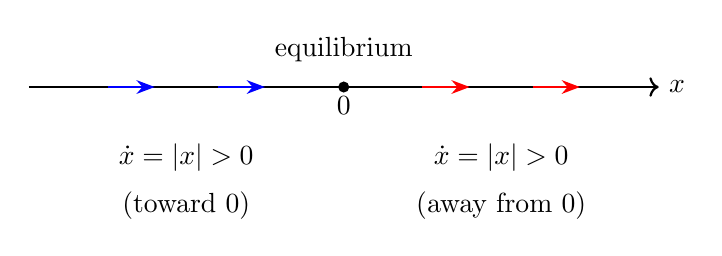
\begin{tikzpicture}[scale=2]
    \draw[->,thick] (-2,0) -- (2,0) node[right] {$x$};
    \fill[black] (0,0) circle (1pt) node[below] {$0$};
    \node[above] at (0,0.1) {equilibrium};

    % Flow arrows
    \draw[-{Stealth},thick,blue] (-1.5,0) -- (-1.2,0);
    \draw[-{Stealth},thick,blue] (-0.8,0) -- (-0.5,0);
    \node[below] at (-1,-0.3) {$\dot{x} = |x| > 0$};
    \node[below] at (-1,-0.6) {(toward 0)};

    \draw[-{Stealth},thick,red] (0.5,0) -- (0.8,0);
    \draw[-{Stealth},thick,red] (1.2,0) -- (1.5,0);
    \node[below] at (1,-0.3) {$\dot{x} = |x| > 0$};
    \node[below] at (1,-0.6) {(away from 0)};
\end{tikzpicture}
\end{center}

The equilibrium at $x = 0$ is semi-stable:
\begin{itemize}
    \item Stable from the left (attracts $x < 0$)
    \item Unstable to the right (repels $x > 0$)
\end{itemize}
\end{explanation}

\end{solution}

\vspace{10pt}
\hrule
\vspace{10pt}

\subsection*{(iii) Uniqueness of Orbits}

\begin{solution}

\textbf{Answer:} \boxed{\text{YES - solutions are unique}}

\begin{explanation}[Why Uniqueness Holds]
For any initial condition $x_0$:
\begin{itemize}
    \item If $x_0 > 0$: unique solution $x(t) = x_0 e^t$
    \item If $x_0 = 0$: unique solution $x(t) = 0$
    \item If $x_0 < 0$: unique solution $x(t) = x_0 e^{-t}$
\end{itemize}

Each solution was obtained by separation of variables in the appropriate region.

At $x = 0$, the solution must stay at zero because $\dot{x} = |0| = 0$.

\textbf{No ambiguity:} The piecewise nature of $|x|$ doesn't create non-uniqueness because solutions starting in one region ($x > 0$ or $x < 0$) never cross to the other region (except by approaching $x = 0$ asymptotically).
\end{explanation}

\end{solution}

\vspace{10pt}
\hrule
\vspace{10pt}

\subsection*{(iv) Lipschitz Continuity}

\begin{solution}

\textbf{Question:} Is $f(x) = |x|$ Lipschitz continuous?

\textbf{Step 1: Compute the Derivative}

$$f'(x) = \frac{d}{dx}|x| = \begin{cases}
+1 & \text{if } x > 0 \\
\text{undefined} & \text{if } x = 0 \\
-1 & \text{if } x < 0
\end{cases}$$

\textbf{Step 2: Check Boundedness of $|f'(x)|$}

For $x \neq 0$: $|f'(x)| = 1$ (bounded!)

But $f'(0)$ does not exist (derivative undefined at origin).

\textbf{Step 3: Direct Lipschitz Test}

For any $x_1, x_2$:
$$|f(x_1) - f(x_2)| = ||x_1| - |x_2||$$

By the reverse triangle inequality:
$$||x_1| - |x_2|| \leq |x_1 - x_2|$$

Therefore:
$$|f(x_1) - f(x_2)| \leq |x_1 - x_2|$$

This holds with Lipschitz constant $L = 1$.

\boxed{\text{YES - globally Lipschitz continuous with } L = 1}

\begin{explanation}[Lipschitz Despite Non-Differentiability]
Even though $f(x) = |x|$ is not differentiable at $x = 0$, it is still Lipschitz continuous!

The key insight:
\begin{itemize}
    \item Lipschitz continuity is about bounding $|f(x_1) - f(x_2)|$
    \item It doesn't require differentiability everywhere
    \item The "corner" at $x = 0$ is "mild" enough to satisfy Lipschitz condition
\end{itemize}

\critical{IMPORTANT DISTINCTION:}
\begin{itemize}
    \item Differentiable + bounded derivative $\Rightarrow$ Lipschitz
    \item But Lipschitz $\not\Rightarrow$ Differentiable everywhere
    \item $|x|$ is Lipschitz but not differentiable at 0
\end{itemize}
\end{explanation}

\textbf{Agreement with (iii):}

\begin{itemize}
    \item $f(x) = |x|$ is Lipschitz continuous $\checkmark$
    \item Picard-Lindelöf theorem guarantees uniqueness $\checkmark$
    \item Solutions are indeed unique $\checkmark$
    \item Perfect agreement! $\checkmark$
\end{itemize}

\end{solution}

\newpage

\section{Part (c): $\dot{x} = |x|^{1/2}$ with $x(0) = x_0$}

\subsection*{Solving the ODE}

\begin{solution}

\textbf{Note:} This problem is provided with the solution in the problem statement. We verify and analyze it.

\textbf{Given Solution:}

$$x(t) = \begin{cases}
+\left(|x_0|^{1/2} + \frac{1}{2}t\right)^2 & \text{if } x_0 \geq 0 \\
0 & \text{if } x_0 = 0 \\
-\left(|x_0|^{1/2} - \frac{1}{2}t\right)^2 & \text{if } x_0 \leq 0
\end{cases}$$

\textbf{Step 1: Verify the Solution for $x_0 > 0$}

Let $x(t) = \left(\sqrt{x_0} + \frac{t}{2}\right)^2$ with $x_0 > 0$

Check initial condition:
$$x(0) = \left(\sqrt{x_0}\right)^2 = x_0 \quad \checkmark$$

Compute derivative:
$$\frac{dx}{dt} = 2\left(\sqrt{x_0} + \frac{t}{2}\right) \cdot \frac{1}{2} = \sqrt{x_0} + \frac{t}{2}$$

Since $x(t) > 0$ for all $t \geq 0$:
$$|x|^{1/2} = \sqrt{x} = \sqrt{\left(\sqrt{x_0} + \frac{t}{2}\right)^2} = \sqrt{x_0} + \frac{t}{2}$$

Therefore $\dot{x} = |x|^{1/2}$ ✓

\textbf{Step 2: Verify the Solution for $x_0 < 0$}

Let $x(t) = -\left(\sqrt{|x_0|} - \frac{t}{2}\right)^2$ with $x_0 < 0$

For $0 \leq t < 2\sqrt{|x_0|}$, we have $x(t) < 0$, so:
$$|x|^{1/2} = \sqrt{-x} = \sqrt{\left(\sqrt{|x_0|} - \frac{t}{2}\right)^2} = \sqrt{|x_0|} - \frac{t}{2}$$

Compute derivative:
$$\frac{dx}{dt} = -2\left(\sqrt{|x_0|} - \frac{t}{2}\right) \cdot \left(-\frac{1}{2}\right) = \sqrt{|x_0|} - \frac{t}{2}$$

Therefore $\dot{x} = |x|^{1/2}$ ✓

\begin{explanation}[Key Observation]
For $x_0 < 0$, the solution $x(t) = -\left(\sqrt{|x_0|} - \frac{t}{2}\right)^2$ reaches zero at time:
$$t^* = 2\sqrt{|x_0|}$$

At this point, the solution becomes $x(t) = 0$ for all $t \geq t^*$.

This is because once $x = 0$, we have $\dot{x} = |0|^{1/2} = 0$, so the solution stays at zero.
\end{explanation}

\end{solution}

\vspace{10pt}
\hrule
\vspace{10pt}

\subsection*{(i) Behavior for Three Initial Conditions}

\begin{solution}

\textbf{Case 1: $x_0 = 0$}

$$x(t) = 0 \quad \text{for all } t$$

\begin{itemize}
    \item \textbf{Where does it go?} Stays at $x = 0$ forever
    \item \textbf{How long?} Remains there for all time
    \item \textbf{Nature:} Equilibrium solution
\end{itemize}

\textbf{Case 2: $x_0 = -1$}

$$x(t) = -\left(1 - \frac{t}{2}\right)^2 \quad \text{for } 0 \leq t \leq 2$$

After $t = 2$: $x(t) = 0$

\begin{itemize}
    \item At $t = 0$: $x = -1$
    \item At $t = 1$: $x = -\left(\frac{1}{2}\right)^2 = -\frac{1}{4}$
    \item At $t = 2$: $x = 0$
    \item For $t \geq 2$: $x = 0$
    \item \textbf{Where does it go?} Reaches $x = 0$ and stays there
    \item \textbf{How long?} Reaches zero in finite time $t^* = 2$
\end{itemize}

\begin{explanation}[Finite-Time Arrival at Zero]
Unlike parts (a) and (b), where solutions from $x_0 < 0$ approach zero asymptotically (taking infinite time), here the solution reaches zero in finite time!

This is because $\dot{x} = |x|^{1/2}$ is a sub-linear growth rate. Near $x = 0$:
$$\frac{dx}{dt} \sim \sqrt{|x|} \to 0 \quad \text{slowly enough that } \int_0^{x_0} \frac{dx}{\sqrt{|x|}} < \infty$$
\end{explanation}

\textbf{Case 3: $x_0 = +1$}

$$x(t) = \left(1 + \frac{t}{2}\right)^2$$

\begin{itemize}
    \item At $t = 0$: $x = 1$
    \item At $t = 2$: $x = (2)^2 = 4$
    \item At $t = 4$: $x = (3)^2 = 9$
    \item As $t \to \infty$: $x(t) \sim \frac{t^2}{4} \to +\infty$
    \item \textbf{Where does it go?} Diverges to $+\infty$
    \item \textbf{How long?} Infinite time (algebraic growth)
    \item Growth rate: $\sim t^2$ (slower than exponential)
\end{itemize}

\textbf{Summary:}

\begin{center}
\begin{tabular}{|c|c|c|}
\hline
$x_0$ & Long-time behavior & Time to destination \\
\hline
$0$ & Stays at $x = 0$ & All time \\
\hline
$-1$ & Reaches $x = 0$ & Finite time ($t^* = 2$) \\
\hline
$+1$ & $x(t) \to +\infty$ & Infinite time \\
\hline
\end{tabular}
\end{center}

\end{solution}

\vspace{10pt}
\hrule
\vspace{10pt}

\subsection*{(ii) Different Orbits}

\begin{solution}

\textbf{Classification of Orbits:}

\textbf{Type 1: Equilibrium Orbit}
$$x(t) = 0 \quad \text{for all } t$$
Starting point: $x_0 = 0$

\textbf{Type 2: Finite-Time Arrival at Zero ($x_0 < 0$)}
$$x(t) = \begin{cases}
-\left(\sqrt{|x_0|} - \frac{t}{2}\right)^2 & \text{for } 0 \leq t \leq 2\sqrt{|x_0|} \\
0 & \text{for } t > 2\sqrt{|x_0|}
\end{cases}$$
\begin{itemize}
    \item Solution increases from $x_0$ to $0$
    \item Reaches zero at time $t^* = 2\sqrt{|x_0|}$
    \item Stays at zero thereafter
\end{itemize}

\textbf{Type 3: Algebraic Growth to Infinity ($x_0 > 0$)}
$$x(t) = \left(\sqrt{x_0} + \frac{t}{2}\right)^2$$
\begin{itemize}
    \item Solution exists for all $t \geq 0$
    \item Grows like $\sim t^2$ for large $t$
    \item $x(t) \to +\infty$ as $t \to \infty$
\end{itemize}

\begin{explanation}[Phase Portrait]
\begin{center}
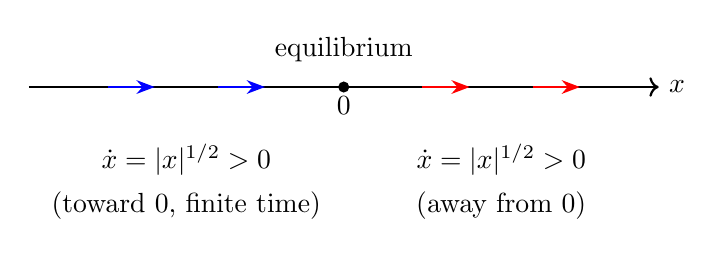
\begin{tikzpicture}[scale=2]
    \draw[->,thick] (-2,0) -- (2,0) node[right] {$x$};
    \fill[black] (0,0) circle (1pt) node[below] {$0$};
    \node[above] at (0,0.1) {equilibrium};

    % Flow arrows
    \draw[-{Stealth},thick,blue] (-1.5,0) -- (-1.2,0);
    \draw[-{Stealth},thick,blue] (-0.8,0) -- (-0.5,0);
    \node[below] at (-1,-0.3) {$\dot{x} = |x|^{1/2} > 0$};
    \node[below] at (-1,-0.6) {(toward 0, finite time)};

    \draw[-{Stealth},thick,red] (0.5,0) -- (0.8,0);
    \draw[-{Stealth},thick,red] (1.2,0) -- (1.5,0);
    \node[below] at (1,-0.3) {$\dot{x} = |x|^{1/2} > 0$};
    \node[below] at (1,-0.6) {(away from 0)};
\end{tikzpicture}
\end{center}

Equilibrium at $x = 0$ is semi-stable, but with a crucial difference from parts (a) and (b): trajectories from $x < 0$ reach the equilibrium in finite time.
\end{explanation}

\end{solution}

\vspace{10pt}
\hrule
\vspace{10pt}

\subsection*{(iii) Uniqueness of Orbits}

\begin{solution}

\textbf{Answer:} \boxed{\text{NO - solutions are NOT unique from } x_0 = 0}

\begin{explanation}[Non-Uniqueness at Origin]

From the initial condition $x(0) = 0$, we have \textbf{infinitely many solutions}!

\textbf{Solution 1: Stay at zero}
$$x(t) = 0 \quad \text{for all } t$$

This clearly satisfies $\dot{x} = |0|^{1/2} = 0$ and $x(0) = 0$.

\textbf{Solution 2: Leave zero at any time $t_0 \geq 0$}

For any $t_0 \geq 0$, define:
$$x(t) = \begin{cases}
0 & \text{for } 0 \leq t \leq t_0 \\
\left(\frac{t - t_0}{2}\right)^2 & \text{for } t > t_0
\end{cases}$$

\textbf{Verification:}
\begin{itemize}
    \item Initial condition: $x(0) = 0$ ✓
    \item For $0 \leq t \leq t_0$: $\dot{x} = 0 = |0|^{1/2}$ ✓
    \item For $t > t_0$: $\dot{x} = 2 \cdot \frac{t-t_0}{2} \cdot \frac{1}{2} = \frac{t-t_0}{2}$ and $|x|^{1/2} = \frac{t-t_0}{2}$ ✓
    \item Continuity at $t = t_0$: $\lim_{t \to t_0^-} x(t) = 0 = \lim_{t \to t_0^+} x(t)$ ✓
    \item Derivative at $t = t_0$: Both sides give $\dot{x} = 0$ ✓
\end{itemize}

So for EVERY choice of $t_0 \geq 0$, we get a different valid solution!

\critical{INFINITELY MANY SOLUTIONS FROM $x_0 = 0$}

This is a fundamental failure of uniqueness.
\end{explanation}

\textbf{From other initial conditions ($x_0 \neq 0$):}

Solutions ARE unique:
\begin{itemize}
    \item If $x_0 > 0$: unique solution $x(t) = \left(\sqrt{x_0} + \frac{t}{2}\right)^2$
    \item If $x_0 < 0$: unique solution given by the piecewise formula
\end{itemize}

The non-uniqueness is localized to $x = 0$.

\end{solution}

\vspace{10pt}
\hrule
\vspace{10pt}

\subsection*{(iv) Lipschitz Continuity}

\begin{solution}

\textbf{Question:} Is $f(x) = |x|^{1/2}$ Lipschitz continuous?

\textbf{Step 1: Compute the Derivative (where it exists)}

For $x > 0$:
$$f(x) = x^{1/2} \quad \Rightarrow \quad f'(x) = \frac{1}{2}x^{-1/2} = \frac{1}{2\sqrt{x}}$$

For $x < 0$:
$$f(x) = (-x)^{1/2} \quad \Rightarrow \quad f'(x) = -\frac{1}{2}(-x)^{-1/2} = \frac{1}{2\sqrt{-x}}$$

At $x = 0$: derivative does not exist.

\textbf{Step 2: Check Boundedness}

$$\lim_{x \to 0^+} f'(x) = \lim_{x \to 0^+} \frac{1}{2\sqrt{x}} = +\infty$$

$$\lim_{x \to 0^-} f'(x) = \lim_{x \to 0^-} \frac{1}{2\sqrt{-x}} = +\infty$$

The derivative is \textbf{UNBOUNDED} near $x = 0$!

\textbf{Step 3: Direct Lipschitz Test}

For Lipschitz continuity, we need:
$$|f(x_1) - f(x_2)| \leq L|x_1 - x_2| \quad \text{for some constant } L$$

Take $x_1 = h > 0$ and $x_2 = 0$ with small $h$:
$$|f(h) - f(0)| = |\sqrt{h} - 0| = \sqrt{h}$$
$$|x_1 - x_2| = |h - 0| = h$$

For Lipschitz: $\sqrt{h} \leq L \cdot h$, which gives $L \geq \frac{\sqrt{h}}{h} = \frac{1}{\sqrt{h}}$

As $h \to 0$: $\frac{1}{\sqrt{h}} \to \infty$

Therefore, no finite $L$ exists!

\boxed{\text{NOT Lipschitz continuous at } x = 0}

\begin{explanation}[Why Not Lipschitz]
The function $f(x) = |x|^{1/2}$ has a "vertical tangent" at $x = 0$:
\begin{itemize}
    \item The slope approaches infinity as we approach the origin
    \item This violates the Lipschitz condition, which requires bounded slopes
    \item The "corner" at $x = 0$ is too sharp
\end{itemize}

Compare to part (b): $|x|$ has a "corner" but finite slope ($\pm 1$), so it's Lipschitz.

Here: $|x|^{1/2}$ has infinite slope at 0, so NOT Lipschitz.
\end{explanation}

\textbf{Agreement with (iii):}

\begin{itemize}
    \item $f(x) = |x|^{1/2}$ is NOT Lipschitz continuous at $x = 0$ $\checkmark$
    \item Picard-Lindelöf theorem does NOT guarantee uniqueness $\checkmark$
    \item Solutions from $x_0 = 0$ are NOT unique $\checkmark$
    \item Perfect agreement! $\checkmark$
\end{itemize}

\critical{THE LIPSCHITZ CONDITION IS CRUCIAL FOR UNIQUENESS}

When the Lipschitz condition fails, uniqueness can fail. This example demonstrates why the Lipschitz condition in the Picard-Lindelöf theorem is not just a technical requirement—it's essential!

\end{solution}

\newpage

\section{Summary and Comparison}

\subsection*{Comparison of All Three Parts}

\begin{center}
\small
\begin{tabular}{|l|c|c|c|}
\hline
\textbf{Property} & \textbf{(a) $\dot{x} = x^2$} & \textbf{(b) $\dot{x} = |x|$} & \textbf{(c) $\dot{x} = |x|^{1/2}$} \\
\hline
\hline
\multicolumn{4}{|c|}{\textbf{Solutions from Different Initial Conditions}} \\
\hline
$x_0 = 0$ & $x(t) = 0$ & $x(t) = 0$ & $x(t) = 0$ (or others!) \\
\hline
$x_0 = -1$ & $\frac{-1}{1+t} \to 0$ & $-e^{-t} \to 0$ & Reaches 0 at $t=2$ \\
\hline
$x_0 = +1$ & $\frac{1}{1-t}$ blows up & $e^t \to \infty$ & $(1+\frac{t}{2})^2 \to \infty$ \\
\hline
\hline
\multicolumn{4}{|c|}{\textbf{Time to Reach Destination}} \\
\hline
From $x_0 = -1$ to 0 & Infinite & Infinite & Finite ($t = 2$) \\
\hline
From $x_0 = +1$ to $\infty$ & Finite ($t = 1$) & Infinite & Infinite \\
\hline
\hline
\multicolumn{4}{|c|}{\textbf{Orbit Types}} \\
\hline
Number of orbit types & 3 & 3 & 3 \\
\hline
Equilibrium & Yes (at 0) & Yes (at 0) & Yes (at 0) \\
\hline
Finite-time blow-up & Yes ($x_0 > 0$) & No & No \\
\hline
Finite-time arrival & No & No & Yes ($x_0 < 0$) \\
\hline
\hline
\multicolumn{4}{|c|}{\textbf{Uniqueness and Lipschitz}} \\
\hline
Unique solutions? & YES & YES & NO (at $x_0=0$) \\
\hline
Globally Lipschitz? & NO & YES & NO \\
\hline
Locally Lipschitz? & YES & YES & NO (at $x=0$) \\
\hline
$f'(x)$ at $x=0$ & $f'(0) = 0$ & Undefined & $+\infty$ \\
\hline
\hline
\multicolumn{4}{|c|}{\textbf{Growth Rates}} \\
\hline
Type & Superlinear & Linear (exp) & Sublinear \\
\hline
$\dot{x}$ for large $x$ & $\sim x^2$ & $\sim x$ & $\sim \sqrt{x}$ \\
\hline
\end{tabular}
\end{center}

\subsection*{Key Insights from This Exercise}

\begin{explanation}[The Role of Lipschitz Continuity]

\textbf{What we learned:}

\begin{enumerate}
    \item \textbf{Sufficient but not necessary:} Lipschitz $\Rightarrow$ uniqueness, but uniqueness doesn't require Lipschitz (see part (a))

    \item \textbf{Local vs. Global:} Local Lipschitz often sufficient for local uniqueness

    \item \textbf{When it fails:}
    \begin{itemize}
        \item Part (c): $f(x) = |x|^{1/2}$ has $f'(0) = \infty$
        \item Result: infinitely many solutions from $x_0 = 0$
        \item The vertical tangent allows "branching" of solutions
    \end{itemize}

    \item \textbf{Differentiability:}
    \begin{itemize}
        \item Part (b): $f(x) = |x|$ not differentiable at 0, but still Lipschitz
        \item Lipschitz is a weaker condition than differentiability
    \end{itemize}
\end{enumerate}

\end{explanation}

\subsection*{Finite-Time Phenomena}

\begin{explanation}[Finite-Time Blow-Up vs. Finite-Time Arrival]

\textbf{Finite-Time Blow-Up (Part a, $x_0 > 0$):}
\begin{itemize}
    \item Growth rate $\dot{x} = x^2$ is superlinear
    \item Solution reaches $+\infty$ in finite time
    \item Example: $x(t) = \frac{1}{1-t}$ blows up at $t = 1$
\end{itemize}

\textbf{Finite-Time Arrival (Part c, $x_0 < 0$):}
\begin{itemize}
    \item Growth rate $\dot{x} = |x|^{1/2}$ is sublinear
    \item Solution reaches 0 in finite time (from below)
    \item Example: $x(t) = -(1 - \frac{t}{2})^2$ reaches 0 at $t = 2$
    \item After arrival, stays at 0 (or can leave—non-uniqueness!)
\end{itemize}

\textbf{Infinite-Time Asymptotic (Part b):}
\begin{itemize}
    \item Growth rate $\dot{x} = |x|$ is linear
    \item Exponential approach/departure
    \item Never reaches destination in finite time
\end{itemize}

\end{explanation}

\subsection*{Mathematical Rigor: What This Exercise Teaches}

\begin{enumerate}
    \item \textbf{Always check assumptions:} Picard-Lindelöf requires Lipschitz—verify it!

    \item \textbf{Non-uniqueness is possible:} Part (c) shows multiple solutions from same IC

    \item \textbf{Finite-time events:} Both blow-up and arrival can occur in finite time

    \item \textbf{Careful case analysis:} Functions like $|x|$ require splitting into cases

    \item \textbf{Verification matters:} Always check solutions satisfy the ODE and IC
\end{enumerate}

\critical{PROFOUND LESSON:} The seemingly small difference between $|x|$ and $|x|^{1/2}$ (both non-smooth at origin) leads to dramatically different behavior regarding uniqueness. The rate of growth near the equilibrium determines whether uniqueness holds!

\vfill

\begin{center}
\Large\textbf{END OF QUESTION 6}
\end{center}

\end{document}
